\section{Обзор существующих библиотек}

В рамках исследования был проведен анализ основных существующих функциональных принтер-библиотек. Все выбранные библиотеки оказались комбинаторными, что естественно для функциональных языков.

% Так как работа проводилась в контексте функциональных языков, для анализа были выбраны комбинаторные библиотеки.
% Комбинаторы естественным образом возникают при наличии в языке функций высших порядков.

\subsection{Модельный язык L}
% \addcontentsline{toc}{section}{Модельный язык L}

В дальнейшем центральным примером, для которого мы будем разрабатывать принтеры, будет модельный язык L. Именно для этого языка будет реализован шаблонный принтер.

Язык L состоит из небольшого числа операторов:
\begin{enumerate}
	\item присваивание;
	\item цикл с предусловием;
	\item ветвление;
	\item последовательное выполнение;
	\item чтение с занесением в переменную;
	\item печать целочисленного выражения.
\end{enumerate}

Также в языке есть выражения. Выражения бывают трех типов:
\begin{enumerate}
	\item константа;
	\item переменная;
	\item бинарная операция.
\end{enumerate}

На рисунке~\ref{fig:lEx} приведен пример программы на языке L. В данном случае, это программа, которая считывает с консоли два числа, а потом возводит второе число в степень, равную первому.

\begin{figure}[h!]
	\centering
	% \inputminted{pascal}{codes/lEx.l}
	\lstinputlisting[language=llang]{codes/lEx.l}
	\caption{Быстрое возведение в степень на языке L}
	\label{fig:lEx}
\end{figure}

\subsection{Библиотека Хьюза}

Библиотека Джона Хьюза\cite{hughes} считается первой комбинаторной принтер-библиотекой. Она основана на алгоритме, предложенном Дереком Оппеном \cite{oppen}, и по сути является его реализацией в функциональном стиле на языке Haskell\footnote{http://haskell.org}. Также библиотека Хьюза, расширенная Саймоном Пейтоном Джонсом \cite{peytonJones}, является стандартной принтер-библиотекой для языка Haskell.

% рассказать об оптимальном

В данной библиотеке ключевым типом является “\lstinline[language=Haskell]{Doc}”. Он представляет документ, который потом может быть переведен в строковое представление.
Основные комбинаторы для составления документа:
% \inputminted{haskell}{Podkopaev/codes/hughesBasicOperators.hs}
\lstinputlisting[language=Haskell]{Podkopaev/codes/hughesBasicOperators.hs}

Так, с помощью функции “\lstinline[language=Haskell]{text}” по строке получается документ, оператор “\textbf{<>}” соединяет два документа горизонтально (см. рисунок~\ref{fig:hughesHorComp}), а оператор “\textbf{\$\$}” соединяет документы вертикально (см. рисунок~\ref{fig:hughesVertComp}).

\begin{figure}[ht]
	\begin{subfigure}[b]{0.45\linewidth}
		\centering
		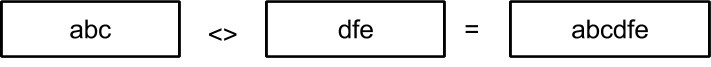
\includegraphics[width=\textwidth]{hughesHorComp}
		\caption{Комбинатор “\textbf{<>}”}
		\label{fig:hughesHorComp}
	\end{subfigure}
	\hspace{0.5cm}
	\begin{subfigure}[b]{0.45\linewidth}
		\centering
		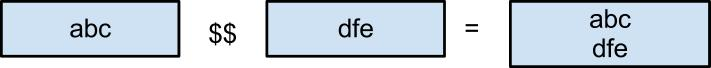
\includegraphics[width=\textwidth]{hughesVertComp}
		\caption{Комбинатор “\textbf{\$\$}”}
		\label{fig:hughesVertComp}
	\end{subfigure}

	\caption{Пример работы комбинаторов}
\end{figure}

Функция “\lstinline[language=Haskell]{nest}” добавляет к каждой строке документа заданное число ведущих пробелов. Функция “\lstinline[language=Haskell]{sep}” является ключевым комбинатором, который в этой библиотеке позволяет задавать плавающую раскладку документа. Она принимает как параметр список документов, а на выходе получается документ, который представляет из себя либо вертикальную склейку элементов списка, либо горизонтальную склейку (в этом случае если к документу из списка применялась функция “\lstinline[language=Haskell]{nest}”, то к этому документу не добавляются ведущие пробелы, то есть применение “\lstinline[language=Haskell]{nest}” попросту игнорируется), причем между документами вставляется пробельный символ. Вариант раскладки выбирается функцией “\lstinline[language=Haskell]{pretty}”:

% \inputminted{haskell}{Podkopaev/codes/hughesPretty.hs}
\lstinputlisting[language=Haskell]{Podkopaev/codes/hughesPretty.hs}

Кроме самого документа, функция “\lstinline[language=Haskell]{pretty}” также принимает два числа: максимальную длину и максимальную наполненность строки. Здесь наполненность строки значит длину текста без ведущих пробельных символов. В ходе работы этой функции и происходит выбор раскладки документа, полученного с помощью комбинатора “\lstinline[language=Haskell]{sep}”. Если горизонтальная раскладка удовлетворяет ограничениям на ширину строки, то она и выбирается. Иначе выбирается вертикальная раскладка.


% Возможно, стоит сделать после обзора всех библиотек

Рассмотрим пример описания принтера с помощью библиотеки Хьюза. Для этого используем учебный язык L. Часть принтера для языка L, отвечающая за представление операторов, показана на рисунке~\ref{fig:lHughesPrinter}.
В примере используется не описанный выше комбинатор “\lstinline[language=Haskell]{<+>}”, который определяется следующим образом:

\lstinputlisting[language=Haskell]{Podkopaev/codes/hughesAddComb.hs}

\begin{figure}[h!]
	% \inputminted{haskell}{Podkopaev/codes/lHughesPrinter.hs}
	\lstinputlisting[language=Haskell]{Podkopaev/codes/lHughesPrinter.hs}
	\caption{Принтер, написанный с помощью библиотеки Хьюза}
	\label{fig:lHughesPrinter}
\end{figure}

В данном случае принтер получился несложным, но абсолютно не наглядным. Поскольку в библиотеке нет механизмов, позволяющих явно варьировать раскладку документа в зависимости от раскладки его поддокументов, невозможно выразить пример с рисунка~\ref{fig:lGoodWriteEx}.
То есть, в случае многострочного выражения в операторе “\lstinline[language=llang]{write}”, напечатать закрывающую скобку на уровне самого оператора.

\begin{figure}[h!]
	% \inputminted{pascal}{Podkopaev/codes/lGoodWriteEx.l}
	\lstinputlisting[language=llang]{Podkopaev/codes/lGoodWriteEx.l}
	\caption{Желательный пример печати конструкции “\lstinline[language=llang]{write}”}
	\label{fig:lGoodWriteEx}
\end{figure}

С помощью реализации принтера с рисунка~\ref{fig:lHughesPrinter}, в данном случае для оператора “\lstinline[language=llang]{write}” получится немного не то (см. рисунок~\ref{fig:lCurWriteEx}).
\begin{figure}[h!]
	% \inputminted{pascal}{Podkopaev/codes/lCurWriteEx.l}
	\lstinputlisting[language=llang]{Podkopaev/codes/lCurWriteEx.l}
	\caption{Результат для изначального принтера конструкции “\lstinline[language=llang]{write}”}
	\label{fig:lCurWriteEx}
\end{figure}

Если попробовать поменять функцию “\lstinline[language=Haskell]{docFromOperation}” для конструкции “\lstinline[language=llang]{write}” (см. рис. \ref{fig:lHughesWriteChange}),
то для многострочного выражения все получится правильно, но в случае однострочного --- появится лишний пробел перед закрывающей скобкой (см. рис. \ref{fig:lBadWriteEx})).

\begin{figure}[h!]
	% \inputminted{haskell}{Podkopaev/codes/lHughesWriteChange.hs}
	\lstinputlisting[language=Haskell]{Podkopaev/codes/lHughesWriteChange.hs}
	\caption{Измененный принтер конструкции “\lstinline[language=llang]{write}”}
	\label{fig:lHughesWriteChange}
\end{figure}

\begin{figure}[h!]
	% \inputminted{pascal}{Podkopaev/codes/lBadWriteEx.l}
	\lstinputlisting[language=llang]{Podkopaev/codes/lBadWriteEx.l}
	\caption{Результат для измененого принтера конструкции “\lstinline[language=llang]{write}”}
	\label{fig:lBadWriteEx}
\end{figure}
\newpage

\subsection{Принтер-комбинаторная библиотека Вадлера}

В \cite{wadler} Филипп Вадлер описал свою комбинаторную бибилиотеку для форматированного вывода на языке Haskell. Она является модификацией библиотеки Хьюза, описанной в предыдущем разделе. Код библиотеки сократился с $\approx$ 110 строк до $\approx$ 80 строк, и, по исследованию Вадлера, на 30\% увеличилась скорость вычисления раскладки документа.

Рассмотрим основые комбинаторы этой библиотеки:
% \inputminted{haskell}{codes/wadlerBasicOperations.hs}
\lstinputlisting[language=Haskell]{codes/wadlerBasicOperations.hs}

Вадлер решил отказаться от двух разных способов соединения документов, оставив лишь горизонтальную склейку. Но для того, чтобы можно было выражать не только однострочные документы, в библиотеке Вадлера появилась функция “\lstinline[language=Haskell]{line}”. Она создает документ, который может быть переведен в символ новой строки или в пробел.
Функция “\lstinline[language=Haskell]{group}” имеет то же назначение, что и оператор “\lstinline[language=Haskell]{sep}” в библиотеке Хьюза, но работает не со списком документов, а с одним документом, и по сути предоставляет альтернативы для алгоритма перевода документа в “\lstinline[language=Haskell]{String}”: в документе, на который подействовал “\lstinline[language=Haskell]{group}”, либо все вхождения “\lstinline[language=Haskell]{line}” заменяются на пробел, либо остаются переводами строки (если они не являются частью вложенных “\lstinline[language=Haskell]{group}”-документов).

В таком виде библиотека потеряла в выразительности, что признается в статье Вадлера. Но кроме потери выразительности, есть еще один серьезный недостаток, возникающий из-за оператора “\lstinline[language=Haskell]{group}”. То, что любой документ им может быть преобразован в однострочный, делает библиотеку неприменимой в некоторых ситуациях. 

Рассмотрим следующий пример. Пусть нам надо написать принтер для языка Python\footnote{http://python.org}. Для конструкции последовательных операторов принтер изображен на рисунке~\ref{fig:pythonPrinter}.
По-другому его написать нельзя --- мы хотим, чтобы последовательные операторы печатались на новых строках. Но если такая конструкция попадет внутрь “\lstinline[language=Haskell]{group}”-документа, то последовательные строчки могут склеиться пробелом, что сделает код некорректным, так как в Python несколько операторов на одной строке должны разделяться символом “;”.

\begin{figure}[h!]
	% \inputminted{haskell}{codes/pythonPrinter.hs}
	\lstinputlisting[language=Haskell]{codes/pythonPrinter.hs}
	\caption{Принтер для последовательных операторов в Python}
	\label{fig:pythonPrinter}
\end{figure}

Так корректный код (см. рисунок~\ref{fig:pythonCode}) может превратиться в некорректный (см. рисунок~\ref{fig:pythonCodeBad}).
\begin{figure}[h!]
	\centering
	\null\hfill
	\subfloat[]{
		\centering
		\lstinputlisting[language=Python]{codes/pythonCode.py}
		\label{fig:pythonCode}	
	}
	\null\hfill
	\subfloat[]{
		\centering
		\lstinputlisting[language=Python]{codes/pythonCodeBad.py}
		\label{fig:pythonCodeBad}
	}
	\hfill
	\null
	\caption{Пример работы принтера для языка Python}
\end{figure}

\newpage

\subsection{Библиотека Азеро и Свиерстры}

Библиотека Азеро и Свиерстры\footnote{
В данном тексте, с целью не усложнять восприятие, изменены обозначения комбинаторов библиотеки Свиерстры на обозначения, подобные тем, что были уже рассмотрены в библиотеке Хьюза. Семантика комбинаторов описана без изменений, согласно оригинальной статье и соответствующей библиотеке.
}, описанная в \cite{swierstra}, отличается от предыдущих библиотек тем, что дает возможность явным образом задать несколько несвязанных вариантов раскладки документа. В этой библиотеке есть комбинатор “\lstinline[language=Haskell]{<|>}”:

% \inputminted{haskell}{Podkopaev/codes/chooseSw.hs}
\lstinputlisting[language=Haskell]{Podkopaev/codes/chooseSw.hs}

Этот комбинатор берет два документа и создает новый, который при раскладке может стать первым или вторым, в зависимости от того, какой из документов раскладывается оптимальней. \textit{Оптимальной} раскладкой для документа считается раскладка, удовлетворяющая ограничению на ширину документа и имеющая минимальную высоту.

Наличие комбинатора “\lstinline[language=Haskell]{<|>}” сразу же решает проблему со скобкой, которая была поднята в обзоре библиотеки Хьюза (см. рис.~\ref{fig:bracketSwierstra}).\footnote{
	В примере используется функция “\lstinline[language=Haskell]{element_h1}”. Эта функция выбирает из вариантов раскладки документа те, которые имеют высоту 1.
}

\begin{figure}[h!]
	% \inputminted{haskell}{Podkopaev/codes/bracketSwierstra.hs}
	\lstinputlisting[language=Haskell]{Podkopaev/codes/bracketSwierstra.hs}
	\caption{Принтер конструкции “\lstinline{write}”, удовлетворяющий примеру с рис.~\ref{fig:lGoodWriteEx}}
	\label{fig:bracketSwierstra}
\end{figure}

% Данная вариативность достигается за счет особого представления документа. В данной библиотеке он представляется как ленивый список раскладок, причем список отсортирован в порядке возрастания количества строк раскладки.

Библиотека Азеро и Свиерстры обладает самым богатым набором комбинаторов и, благодаря оператору “\lstinline[language=Haskell]{<|>}”, позволяет выразить практически любые принтеры. Но, также как остальные рассмотренные библиотеки, не дает механизмов для простого и наглядного задания принтеров.